% Generated from the public primitive catalog. Original Atlas drawing; Apache-2.0.
% Target: chacha20-poly1305; view: overview-compact
\documentclass[border=9pt]{standalone}
% Original Atlas figure theme. Apache-2.0; see the repository LICENSE.
\usepackage[T1]{fontenc}
\usepackage{lmodern}
\usepackage{amsmath,amssymb}
\usepackage{tikz}
\usetikzlibrary{arrows.meta,positioning,calc,fit,backgrounds,decorations.pathreplacing,matrix}
\definecolor{atlasInk}{HTML}{172235}
\definecolor{atlasTeal}{HTML}{0D7B7D}
\definecolor{atlasMuted}{HTML}{637278}
\definecolor{atlasFill}{HTML}{EAF4F2}
\definecolor{atlasLine}{HTML}{B6C8C7}
\tikzset{
  every picture/.style={line width=.65pt,draw=atlasInk,>=Latex},
  every node/.style={text=atlasInk,font=\sffamily\small},
  box/.style={draw,rounded corners=1.5pt,minimum height=.9cm,minimum width=1.6cm,align=center,inner sep=6pt,fill=white},
  accent/.style={box,draw=atlasTeal,fill=atlasFill},
  wire/.style={->,line width=.7pt},
  keywire/.style={wire,draw=atlasTeal,dashed},
  xor/.style={draw,circle,fill=white,inner sep=0pt,minimum size=.38cm},
  add/.style={draw,rectangle,fill=white,inner sep=0pt,minimum size=.38cm},
  note/.style={font=\sffamily\scriptsize,text=atlasMuted,align=center},
  phase/.style={font=\sffamily\small\bfseries,text=atlasTeal},
  group/.style={draw=atlasLine,dashed,rounded corners=2pt,inner sep=8pt}
}
\newcommand{\rotl}{\mathbin{\lll}}
\newcommand{\rotr}{\mathbin{\ggg}}
\newcommand{\kx}{\operatorname{Keccak}\!\text{-}\!f[1600]}

\newcommand{\AtlasKeyBits}{256}
\newcommand{\AtlasKeyWords}{8}
\newcommand{\AtlasRounds}{N_r}
\newcommand{\AtlasPriorRounds}{N_r-1}
\newcommand{\AtlasRoundKeys}{N_r+1}
\newcommand{\AtlasDoubleRounds}{N_r/2}
\newcommand{\AtlasSixRoundGroups}{N_r/6}
\newcommand{\AtlasFLGroups}{N_r/6-1}
\newcommand{\AtlasRoundStart}{24-n}
\newcommand{\AtlasBlockBits}{b}
\newcommand{\AtlasOutputBits}{d}
\newcommand{\AtlasStateBits}{8w}
\newcommand{\AtlasNonceBits}{96}
\newcommand{\AtlasCounterBits}{q}
\newcommand{\AtlasStreamBlockBits}{b}
\newcommand{\AtlasRate}{r}
\newcommand{\AtlasCapacity}{c}
\newcommand{\AtlasSteps}{N}
\newcommand{\AtlasLastStep}{N-1}
\newcommand{\AtlasWordBits}{w}
\newcommand{\AtlasHashWords}{h}
\newcommand{\AtlasFeedForward}{\boxplus}
\newcommand{\AtlasByteOrder}{big-endian}
\newcommand{\AtlasDomain}{01}
\newif\ifAtlasXof
\AtlasXoffalse
\begin{document}
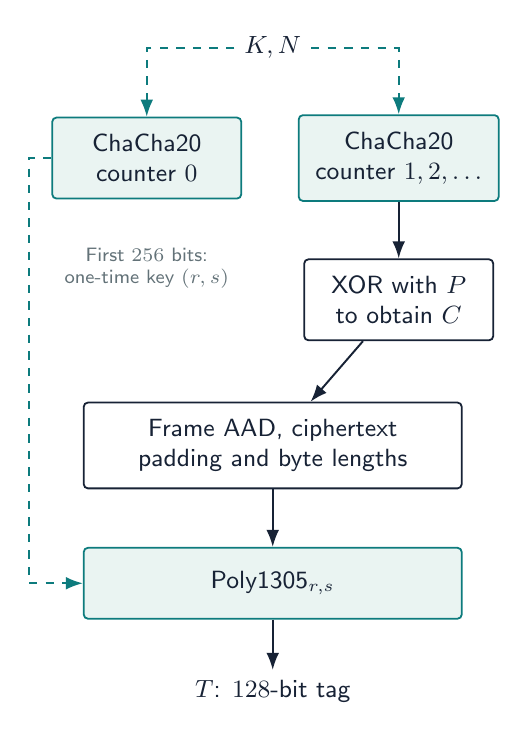
\begin{tikzpicture}
  \node (input) at (0,1.2) {$K,N$};
  \node[accent,minimum width=2.4cm] (otk) at (-1.6,-.2) {ChaCha20\\counter $0$};
  \node[accent,minimum width=2.4cm] (enc) at (1.6,-.2) {ChaCha20\\counter $1,2,\ldots$};
  \draw[keywire] (input) -| (otk); \draw[keywire] (input) -| (enc);
  \node[note,text width=2.5cm] at (-1.6,-1.6) {First $256$ bits:\\one-time key $(r,s)$};
  \node[box,minimum width=2.4cm] (cipher) at (1.6,-2) {XOR with $P$\\to obtain $C$};
  \draw[wire] (enc) -- (cipher);
  \node[box,minimum width=4.8cm] (frame) at (0,-3.85) {Frame AAD, ciphertext\\padding and byte lengths};
  \draw[wire] (cipher) -- (frame);
  \node[accent,minimum width=4.8cm] (poly) at (0,-5.6) {Poly1305$_{r,s}$};
  \draw[wire] (frame) -- (poly);
  \draw[keywire] (otk.west) -- (-3.1,-.2) |- (poly.west);
  \draw[wire] (poly) -- (0,-6.7) node[below] {$T$: $128$-bit tag};
\end{tikzpicture}

\end{document}
